% Тип документа
\documentclass[a4paper,14pt]{extarticle}

% Шрифты, кодировки, символьные таблицы, переносы
\usepackage{cmap}
\usepackage[T2A]{fontenc}
\usepackage[utf8x]{inputenc}
\usepackage[russian]{babel}

\usepackage
	{
		% Дополнения Американского математического общества (AMS)
		amssymb,
		amsfonts,
		amsmath,
		amsthm,
		physics,
		% Графики и рисунки
		graphicx,
		color,
		geometry,
		multicol,
		tikz,
		wrapfig
	}  
\usepackage[hidelinks]{hyperref}


% Увеличенный межстрочный интервал, французские пробелы
\linespread{1.3} 
\frenchspacing 


\geometry		
	{
		left			=	1cm,
		right 			=	1cm,
		top 			=	2cm,
		bottom 			=	2cm,
		bindingoffset	=	0cm
	}
\usepackage{fancyhdr}
\pagestyle{fancy}
\fancyhf{}
\rhead{Сарафанов Ф.Г.}
\chead{Экзамен по радиоэлектронике, зима 2019}
\lhead{Типовые задачи}
\cfoot{\thepage}


\usepackage{mathrsfs} % буква для обозначения ЭДС 
\newcommand{\eds}{\ensuremath{\mathscr{E}}} % новая команда \EDS для символа


%%%%%%%%%%%%%%%%%%%%%%%%%%%%%%%%%%%%%%%%%%%%%%%%%%%%%%%%%%%%%%%%%%%%%%%%%%%%%%%
\gdef\rot{\operatorname{rot}} \gdef\div{\operatorname{div}}
% \gdef\E{\vec{E}}
% \gdef\D{\vec{D}}
% \gdef\H{\vec{H}}
% \gdef\B{\vec{B}}
% \gdef\j{\vec{j}}
% \gdef\n{\vec{n}}

\gdef\LT{\risingdotseq}
\gdef\out{\text{вых}}
\gdef\in{\text{вх}}
\gdef\newint{\int\limits_{-\infty}^{+\infty}}

\usepackage{lipsum}  
\usepackage{ifthen}
\newcommand{\frc}[2]{\raisebox{2pt}{$\displaystyle#1$}\big/\raisebox{-3pt}{$\displaystyle#2$}}
\usepackage{mathtools}  
\mathtoolsset{showonlyrefs}  
% \usepackage[export]{adjustbox}
\usepackage{cancel}
\DeclareMathAlphabet{\mymathbb}{U}{BOONDOX-ds}{m}{n}
\gdef\H{\mymathbb{1}}

\theoremstyle{definition}
\newtheorem*{task}{Дано}

% №№№№№№№№№№№№№№№№№№№№№№№№№№№№№№№№№№№№№№№№№№№№№№№№№№№№№№№№№№№№№№№№№№№№№№№№№№№№№№№№№№№№№№№№№№№№№№№№№№№№№№№№№№№№
% №№№№№№№№№№№№№№№№№№№№№№№№№№№№№№№№№№№№№№№№№№№№№№№№№№№№№№№№№№№№№№№№№№№№№№№№№№№№№№№№№№№№№№№№№№№№№№№№№№№№№№№№№№№№
\begin{document}
% №№№№№№№№№№№№№№№№№№№№№№№№№№№№№№№№№№№№№№№№№№№№№№№№№№№№№№№№№№№№№№№№№№№№№№№№№№№№№№№№№№№№№№№№№№№№№№№№№№№№№№№№№№№№
% №№№№№№№№№№№№№№№№№№№№№№№№№№№№№№№№№№№№№№№№№№№№№№№№№№№№№№№№№№№№№№№№№№№№№№№№№№№№№№№№№№№№№№№№№№№№№№№№№№№№№№№№№№№№


% %!TEX root = ../problems.tex
\begin{titlepage}
\thispagestyle{empty}
% \centering
\begin{center}
	
{\small\textsc{Нижегородский государственный университет имени Н.\,И. Лобачевского}}
\vskip 3pt \hrule \vskip 5pt
{\small\textsc{Радиофизический факультет}}

\vfill

\begin{spacing}{2}
{\Huge \bf  Типовые задачи радиоэлектроники}\\%\vspace{1em}
\end{spacing}
% \vfill
% \\
\vspace{1em}
{\Large Сарафанов Ф.Г., Платонова М.В., Понур К.А., \\ Карусевич А.А., Шиков А.П., Сидоров Д.А.}\\[2em]
{\large sfg180@yandex.ru}\\
\vspace{1em}
\end{center}

\textbf{Disclaimer.} В данном документе нами собраны решения типовых задач по радиэлектронике, изученные на 3 курсе радиофизического факультета ННГУ. Документ призван облегчить подготовку к зачетам и экзаменам и восполнить пробелы в знаниях читателя по методам решения элементарных задач радиоэлектроники. Разрешено копирование и распространение данного документа с обязательным указанием первоисточника. 
	

	% {Сарафанов Ф.Г., Понур К.А. }%\vskip 12pt Принял:\\ Менсов С.\,Н.}
\begin{center}
	
\vfill
	
	 \today\\Нижний Новгород
\end{center}

\end{titlepage}




\section{Таблица простейших преобразований Лапласа}
\begin{center}
\renewcommand{\arraystretch}{1.7}
\begin{tabular}{| c | c |}
	\hline
	Изображение                         & Оригинал($\displaystyle t\geq0$)              \\[0.9em] \hline
	$\displaystyle1$			                                & $\displaystyle\delta(t)$                     \\ \hline
	$\displaystyle\frac1p$	                          & $\displaystyle1(t)$                          \\[0.9em] \hline
	$\displaystyle\frac{1}{p^2}$                     & $\displaystyle t$                              \\[0.9em] \hline
	$\displaystyle\frac{1}{p+a}$                     & $\displaystyle e^{-at}$                       \\[0.9em] \hline
	$\displaystyle\frac{1}{(p+a)^2}$                 & $\displaystyle te^{-at}$                      \\[0.9em] \hline
	$\displaystyle\frac{p}{p+a}$                     & $\displaystyle\delta(t)-ae^{-at}$            \\[0.9em] \hline
	$\displaystyle\frac{p}{(p+a)^2}$                 & $\displaystyle(1-at) e^{-at}$                \\[0.9em] \hline
	$\displaystyle\frac{a}{p(p+a)}$                  & $\displaystyle1-e^{-at}$                     \\[0.9em] \hline
	$\displaystyle\displaystyle\frac{1}{(p+a)(p+b)}$ & $\displaystyle\frac{1}{b-a} (e^{-at} -e^{-bt} ) $   \\[0.9em] \hline
	$\displaystyle\frac{p}{(p+a)(p+b)}$              & $\displaystyle\frac{1}{b-a} (be^{-bt} -ae^{-at} ) $ \\[0.9em] \hline
	$\displaystyle\frac{b^2}{p^2(p+b)}$              & $\displaystyle bt-(1-e^{-bt})$                \\[0.9em] \hline
	$\displaystyle\frac{\omega}{p^2+\omega^2}$       & $\displaystyle\sin{\omega t}$                \\[0.9em] \hline
	$\displaystyle\frac{p}{p^2+\omega^2}$            & $\displaystyle\cos{\omega t}$ 	            \\[0.9em] \hline
\end{tabular}
\end{center}
\newpage
\section{Типовые задачи по радиоэлектронике}

\subsection{Задача №1}
\begin{task}
	Найти спектр сигнала $S(t)=A\cdot e^{-\frac{t^2}{\tau^2}}$. Нарисовать график $|S(\omega)|$. Что будет при разных $\tau$?
\end{task}
\begin{proof}[\rm{\textbf{Решение}}]
	\^S$(\omega)=A\int\limits_{-\infty}^{+\infty}e^{-\frac{t^2}{\tau^2}}e^{-i\omega t}dt=A\int\limits_{-\infty}^{+\infty}e^{-\qty(\frac{t^2}{\tau^2}+i\omega t)}dt$

	Выделим полный квадрат в степени экспоненты:
	\begin{equation}
		\text{\^S}(\omega) = A\int\limits_{-\infty}^{+\infty}e^{-\qty(\frac{t}{\tau}+\frac{i\omega \tau}{2})^2-\frac{\omega^2 \tau^2}{4}}dt
	\end{equation}
	Сделаем замену переменных: $\frac{t}{\tau}+\frac{i\omega \tau}{2} = x$ , $t=\tau x-\frac{i\omega \tau}{2}\tau$ , $dt=\tau dx$
	\begin{equation}
		\text{\^S}(\omega)=A\tau e^{\frac{-\omega^2 \tau^2}{4}} \int\limits_{-\infty}^{+\infty}e^{-x^2}dx
	\end{equation}
	Это интеграл Пуассона, тогда: 
	\begin{equation}
		\text{\^S}(\omega)=A\tau e^{\frac{-\omega^2 \tau^2}{4}} \frac{\sqrt{\pi}}{2}
	\end{equation}

	Чем медленнее изменяется U(t) (т.е. чем больше $\tau$ ), тем быстрее изменяется $|S(\omega)|$ (т.е. тем уже спектр сигнала), и наоборот.
	Похоже ли это на интеграл Пуассона? Наверное, не должно быть деления на 2
\end{proof}
\newpage

\subsection{Задача №2}
%!TEX root = ../problems.tex

\begin{task}
Определить отклик выхода RL-цепи, изображенной на рисунке, на воздействие прямоугольного импульса длительностью $\tau_0$. Нарисовать график $u_\out\qty(t)$. При выполнении какого условия будет осуществляться приближенное интегрирование входной цепи? 
\end{task}

\begin{proof}[\rm{\textbf{Решение}}]
Эквивалентная схема (картиночка)
 \begin{equation}
	u_\in\qty(t)\risingdotseq \frac{A}{p}-\frac{A}{p}\cdot e^{-p\tau}=\frac{A}{p}\qty(1-e^{-p\tau})
\end{equation}
По второму правилу Кирхгофа, сумма падений напряжения на всех элементах цепи равна ЭДС. В нашем случае возможное начальное напряжение на катушке мы относим к ЭДС, а сумму падений напряжения записываем как ток в контуре на суммарный импеданс контура:
\begin{equation}
	\eds=Z(p)\cdot I(p) \quad \Rightarrow \quad
	\frac{A}{p} \qty(1-e^{-p\tau}) + i_L\qty(0)L=\qty(pL+R)I\qty(p)
\end{equation}
Отсюда выражаем ток в контуре:
\begin{equation}
	I\qty(p)=\frac{\frac{A}{p}\qty(1-e^{-p\tau})}{pL+R} + 
		\frac{i_L\qty(0)L}{pL+R}
\end{equation}
% С другой стороны, $u_\in=u_R+u_L$, и отсюда
% \begin{gather}
% \frac{A}{p}\qty(1-e^{-p\tau})=
% 	I\qty(p)R+u_L\qty(p) \Rightarrow \\
% %
% u_L\qty(p) = 
% 	\frac{A}{p}\qty(1-e^{-p\tau})-I\qty(p)R =
% 	\frac{A}{p}\qty(1-e^{-p\tau}) - 
% 		\frac{\frac{AR}{p}\qty(1-e^{-p\tau})}{pL+R} - 
% 		\frac{i_L\qty(0)LR}{pL+R} = \\ =
% %
% \frac{A}{p}\qty(1-e^{-p\tau}) - 
% 	\frac{A\frac{R}{L}}{p\qty(p+\frac{R}{L})} + 
% 	\frac{A\frac{R}{L}}{p\qty(p+\frac{R}{L})}e^{-p\tau} - 
% 	\frac{i_L\qty(0)R}{p+\frac{R}{L}} \LT \\ \LT
% %  
% \cancel{A\H\qty(t)}-
% 	\cancel{A\H\qty({t}-\tau)}-
% 	A\qty(\cancel{1}-e^{-\frac{Rt}{L}}) \H\qty(t) +
% 	A\qty(\cancel{1}-e^{-\frac{R}{L}\qty(t-\tau)}) \H\qty(t-\tau) - 
% 	i_L\qty(0)Re^{\frac{-R}{L}t} \H\qty(t) = \\=
% %
% Ae^{-\frac{Rt}{L}}\cdot \H\qty(t)-
% 	Ae^{-\frac{R\qty(t-\tau)}{L}}\cdot \H\qty(t-\tau)-
% 	i_L\qty(0)Re^{-\frac{Rt}{L}}\cdot \H\qty(t)
% \end{gather}
% Отсюда получаем окончательно выражение для напряжения на индуктивности:
% \begin{equation}
% u_L\qty(t)=
% \qty(A-i_L\qty(0)R)e^{-\frac{Rt}{L}}\cdot \H\qty(t) - 
% 	Ae^{-\frac{R\qty(t-\tau)}{L}}\cdot \H\qty(t-\tau)
% \end{equation}
% Нам надо
Теперь мы можем найти и выходное напряжение -- напряжение на резисторе:
\begin{gather}
	u_\out (p) \equiv u_R\qty(p)=I\qty(p)R=
		\frac{AR\qty(1-e^{-p\tau})}{p\qty(pL+R)}+
		\frac{i_L\qty(0)RL}{pL+R}=
	\frac{\frac{AR}{L}\qty(1-e^{-p\tau})}{p\qty(p+\frac{R}{L})}+
		\frac{i_L\qty(0)R}{p+\frac{R}{L}} 
		=\\=
	A\frac{\frac{R}{L}}{p\qty(p+\frac{R}{L})}-
		A\frac{\frac{R}{L}}{p\qty(p+\frac{R}{L})}e^{-p\tau}+
		i_L\qty(0)R\frac{1}{p+\frac{R}{L}} 
		% \LT \\ \LT 
	% A\qty(1-e^{-\frac{Rt}{L}})\cdot \H\qty(t)-
		% A\qty(1-e^{-\frac{R\qty(t-\tau)}{L}})\cdot \H\qty(t-\tau)+
		% i_L\qty(0)Re^{-\frac{Rt}{L}}\cdot \H\qty(t)
\end{gather}
Используя свойства преобразования Лапласа
\begin{gather}
	\frac{\alpha}{p(p+\alpha)}\LT (1-e^{-\alpha t})\H(t)\\
	\frac{1}{(p+\alpha)}\LT e^{-\alpha t}\H(t)\\
	e^{{-p\tau}}F(p) \LT f(t-\tau)\H(t-\tau), \qq{где} F(p) \LT f(t)
\end{gather}
Из выражения $u_\out(p)$ элементарно получаем оригинал $u_\out(t)$:
\begin{equation}
	u_\out(t)=A\qty(1-e^{-\frac{Rt}{L}})\cdot \H\qty(t)-
		A\qty(1-e^{-\frac{R\qty(t-\tau)}{L}})\cdot \H\qty(t-\tau)+
		i_L\qty(0)Re^{-\frac{Rt}{L}}\cdot \H\qty(t)
\end{equation}
\paragraph{Условие интегрирования.} 
\begin{gather}
	% u_\out\qty(t)=A\qty(1-e^{-\frac{Rt}{L}})\cdot \H\qty(t)-A\qty(1-e^{-\frac{R\qty(t-\tau)}{L}})\cdot \H\qty(t-\tau)+i_L\qty(0)Re^{-\frac{Rt}{L}}\cdot \H\qty(t) 
% \\\tau?>>\tau |\frac{L}{R}>>\tau_| 
\end{gather}
\end{proof}
\newpage

\subsection{Задача №3}
%!TEX root = ../problems.tex
\begin{figure}[h!]
\centering
\begin{minipage}{0.4\textwidth}
\centering
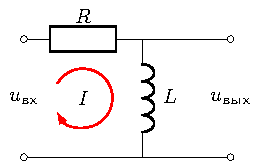
\includegraphics[width=\linewidth]{chem/task3}
\caption{$RL$--контур}
\label{fig:2figsA}
\end{minipage}
\qquad
\begin{minipage}{0.4\textwidth}
\centering
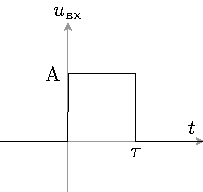
\includegraphics[width=\linewidth]{ris/task2_input}
\caption{Входное напряжение}
\label{fig:2figsB}
\end{minipage}
\end{figure}
\begin{task}
	Определите отклик $u_\out(t)$ $RL$-цепи, изображенной на рисунке, на воздействие единичного импульса длительностью $\tau$. 
	Нарисуйте график отклика. 
	Какова переходная характеристика цепи? 
	При выполнении какого условия будет осуществляться приближённое дифференцирование входной цепи?
	Решить задачу с ненулевыми начальными условиями.
\end{task}
\begin{proof}[\rm{\textbf{Решение}}]
Найдем образ входного импульса преобразованием Лапласа: 
\begin{equation}
	u_\in(t)=E\cdot\H(t)-E\cdot\H(t-\tau)
	\quad\Rightarrow\quad
	u_\in(t)\LT \frac{E}{p}-\frac{E}{p}e^{-p\tau}=
	\frac{E}{p}\qty(1-e^{-p\tau})
\end{equation}
Надо учесть, что в контуре могут быть заданы начальные условия - ток $i_0$.
Тогда начальное напряжение на катушке $u_L(0)=i_0\cdot pL$, а его образ $u_L(0) \LT \frac{i_0 pL}{p}=i_0L$. 
Это напряжение можно трактовать как часть ЭДС.

Обозначим суммарный ток в контуре за $I(p)$. Тогда, так как сумма падений напряжения на каждом элементе равна нулю, получим следующее выражение:
\begin{equation}
	\frac{E}{p}\qty(1-e^{-p\tau})+i_0L=(R+pL)I(p)
\end{equation}
Откуда выразим ток $I$:
\begin{equation}
	I(p)=\frac{\frac{E}{p}\qty(1-e^{-p\tau})+i_0L}{R+pL}
\end{equation}
С другой стороны, $u_\in=u_C+u_R$, а $u_C\equiv u_\out$, тогда
\begin{gather}
	u_\out(p)=u_\in(p)-u_R(p)=u_\in(p)-I(p)R=\\=
	u_\in(p)-\frac{E(1-e^{-p\tau})R}{p(R+pL)}+\frac{i_0LR}{R+pL}=
	u_\in(p)-\frac{ER}{p(R+pL)}+\frac{ERe^{-p\tau}}{p(R+pL)}-\frac{i_0LR}{R+pL}=\\=
	u_\in(p)-\frac{E\frac{R}{L}}{p(p+\frac{R}{L})}+\frac{E\frac{R}{L}e^{-p\tau}}{p(p+\frac{R}{L})}-\frac{i_0R}{p+\frac{R}{L}}
\end{gather}
Используем свойства преобразования Лапласа:
\begin{gather}
	\frac{\alpha}{p(p+\alpha)}\LT (1-e^{-\alpha t})\H(t)\\
	\frac{1}{(p+\alpha)}\LT e^{-\alpha t}\H(t)\\
	e^{{-p\tau}}F(p) \LT f(t-\tau)\H(t-\tau), \qq{где} F(p) \LT f(t)
\end{gather}
Учтя, что $u_\in(p) \LT u_\in(t)$, произведем преобразование:
\begin{gather}
	u_\out(t)=u_\in(t)-E(1-e^{-\frac{R}{L} t})\H(t)+E(1-e^{-\frac{R}{L} (t-\tau)})\H(t-\tau)-i_0Re^{-\frac{R}{L} t}\H(t)=\\=
	\cancel{E\cdot\H(t)}-\cancel{E\cdot\H(t-\tau)}-E(\cancel{1}-e^{-\frac{R}{L} t})\H(t)+E(\cancel{1}-e^{-\frac{R}{L} (t-\tau)})\H(t-\tau)-i_0Re^{-\frac{R}{L} t}\H(t)=\\=\qty(E-i_0R)e^{-\frac{R}{L} t}\H(t)-Ee^{-\frac{R}{L}(t-\tau)}\H(t-\tau)
\end{gather}
Окончательно получили ответ: при воздействии прямоугольным импульсом $u_\in(t)$ амплитуды $E$ и длительностью $\tau$, на выходе получаем
\begin{equation}
 	u_\out(t)= \qty(E-i_0R)e^{-\frac{R}{L} t}\H(t)-Ee^{-\frac{R}{L}(t-\tau)}\H(t-\tau)
\end{equation} 
\paragraph{Условие дифференцирования.} 
Как нетрудно догадаться,
\begin{equation}
	u_\in=u_L+u_R=L\dv{I}{t}+IR
\end{equation}
Продифференцируем это выражение:
\begin{equation}
	\dv{u_\in}{t}=\underbrace{L\dv[2]{I}{t}}_{\dv{u_L}{t}}+\frac{R}{L}\underbrace{L\dv{I}{t}}_{u_L\equiv u_\out}
\end{equation}
Если будет выполнено условие
\begin{equation}
	\abs{\dv{u_L}{t}} \ll \abs{\frac{R}{L} u_L}
\end{equation}
Тогда будет видно, что цепочка осуществляет дифференцирование:
\begin{equation}
	u_\out=\tau_\text{цепи}\dv{u_\in}{t}
\end{equation}
где $\tau_\text{цепи}=\frac{L}{R}$.

Выясним смысл неравенства модулей на примере гармонических сигналов. Пусть входное напряжение гармоническое $u_\in=u_0e^{j\omega t}$. Тогда ток в контуре: $I=I_0e^{j\omega t}$, где $I_0=\frac{u_0}{j\omega L+R}$, и неравенство можно переписать (учтем, что $u_L=I\cdot j\omega L=I_0 j\omega L e^{j\omega t}$):
\begin{equation}
	\abs{I_0\cdot j\omega L\cdot j\omega\cdot e^{j\omega t}}\ll
		\abs{\frac{1}{\tau_\text{цепи}}I_0 \cdot j\omega L\cdot e^{j\omega t}}
	\quad \Rightarrow \quad
	\omega \ll {\frac{1}{\tau_\text{цепи}}}
	\quad \Rightarrow \quad
	T \gg \tau_\text{цепи}
\end{equation}
Таким образом, дифференцирование сигнала <<чистое>> для таких частот, период которых много больше постоянной времени цепи. Отсюда следует <<вилка выбора>> дифференцирующей цепочки: если мы будем расширять частотный диапазон <<чистого>> дифференцирования уменьшением постоянной времени, то амплитуда на выходе цепочки будет падать, и наоборот.
\end{proof}
\newpage

\subsection{Задача №4}
%!TEX root = ../problems.tex
\begin{figure}[h!]
\centering
\begin{minipage}{0.4\textwidth}
\centering
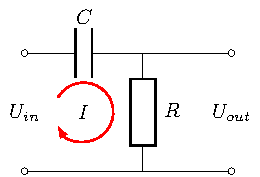
\includegraphics[width=\linewidth]{chem/task4}
\caption{$RC$--контур}
\label{fig:4figsA}
\end{minipage}
\qquad
\begin{minipage}{0.4\textwidth}
\centering
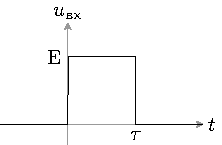
\includegraphics[width=\linewidth]{ris/task4_input}
\caption{Входное напряжение}
\label{fig:4figsB}
\end{minipage}
\end{figure}

\begin{task}
	Определить отклик $u_\out(t)$ $RC$-цепи, изображенной на рисунке, на воздействие прямоугольного импульса длительностью $\tau$. 
	Нарисуйте график отклика. 
	Какова переходная характеристика цепи? 
	При выполнении какого условия будет осуществляться приближённое дифференцирование входной цепи?
	Решить задачу с ненулевыми начальными условиями.
\end{task}
\begin{proof}[\rm{\textbf{Решение}}]
Найдем образ входного импульса преобразованием Лапласа: 
\begin{equation}
	u_\in(t)=E\cdot\H(t)-E\cdot\H(t-\tau)
	\quad\Rightarrow\quad
	u_\in(t)\LT \frac{E}{p}-\frac{E}{p}e^{-p\tau}=
	\frac{E}{p}\qty(1-e^{-p\tau})
\end{equation}
Надо учесть, что в контуре могут быть заданы начальные условия - напряжение на конденсаторе $u_C(0)=u_0$. Его образ $u_C(0) \LT \frac{u_0}{p} $

Обозначим суммарный ток в контуре за $I(p)$. Тогда, так как сумма падений напряжения на каждом элементе равна нулю, получим следующее выражение:
\begin{equation}
	\frac{E}{p}\qty(1-e^{-p\tau})=(R+\frac{1}{pC})I(p)+\frac{u_0}{p}
\end{equation}
Откуда выразим ток $I$:
\begin{equation}
	I(p)=\frac{\frac{E}{p}\qty(1-e^{-p\tau})+u_0/p}{R+\frac{1}{pC}}
\end{equation}
После простых алгебраических преобразований получим:
\begin{equation}
	I(p)=
	\frac{\frac ER }{p+\frac{1}{RC}}-
	\frac{\frac ER e^{-p\tau}}{p+\frac{1}{RC}}-
	\frac{\frac{u_0}R}{p+\frac{1}{RC}}
\end{equation}
Используем свойства преобразования Лапласа:
\begin{gather}
	\frac{\alpha}{p(p+\alpha)}\LT (1-e^{-\alpha t})\H(t)\\
	\frac{1}{(p+\alpha)}\LT e^{-\alpha t}\H(t)\\
	e^{{-p\tau}}F(p) \LT f(t-\tau)\H(t-\tau), \qq{где} F(p) \LT f(t)
\end{gather}
Произведем преобразование:
\begin{gather}
	I(t)=(E-u_0)\frac{\H(t)}{R}\exp{-\frac{t}{RC}}-\frac ER \exp{-\frac{t- \tau	}{RC}}\H(t-\tau )
\end{gather}

Воспользуемся соотношением $u\out=I(t)R$ и окончательно получили ответ: при воздействии прямоугольным импульсом $u_\in(t)$ амплитуды $E$ и длительностью $\tau$, на выходе получаем
\begin{figure}[h!]
	\centering
	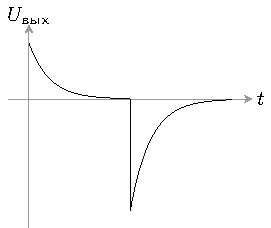
\includegraphics[scale=1.5]{ris/task4_out2}
	\caption{Решение при $E=1, u_0=0.5, \tau=5$}
	\label{fig:4.2}
\end{figure}

\begin{equation}
	u(t)=(E-u_0)\H(t)\exp{-\frac{t}{RC}}-E \exp{-\frac{t- \tau	}{RC}}\H(t-\tau )
\end{equation} 
График решения при $E=1, u_0=0.5, \tau=5$ изображен на рис. \ref{fig:4.2}


\paragraph{Условие дифференцирования.} 
Как нетрудно догадаться,
\begin{equation}
	u_\in=u_C+u_R=\frac{q}{C}+IR
\end{equation}
Продифференцируем это выражение:
\begin{equation}
	\dv{u_\in}{t}=
	\frac{1}{RC}\underbrace{IR}_{u_R\equiv u_\out}+
	\underbrace{\dv{I}{t}R}_{\dv{u_R}{t}}
\end{equation}
Если будет выполнено условие
\begin{equation}
	\abs{\dv{u_R}{t}} \ll \abs{\frac{1}{RC} u_R}
\end{equation}
Тогда будет видно, что цепочка осуществляет дифференцирование:
\begin{equation}
	u_\out=RC\dv{u_\in}{t}=\tau_{\text{цепи}}\dv{u_\in}{t}
\end{equation}




Выясним смысл неравенства модулей на примере гармонических сигналов. Пусть входное напряжение гармоническое $u_\in=u_0e^{i\omega t}$. Тогда ток в контуре: $I=I_0 e^{i\omega t}$, где $I_0=\frac{u_0}{\frac{1}{i \omega C}+R}$, и неравенство можно переписать (учтем, что $u_C=\frac{I}{i \omega C}=\frac{I_0e^{i \omega t}}{i \omega C}$):
\begin{equation}
	\abs{ I_0R \cdot i\omega\cdot e^{i\omega t}}\ll
		\abs{\frac{1}{\tau_\text{цепи}}{I_0}R \cdot e^{i\omega t}}
	\quad \Rightarrow \quad
	\omega \ll {\frac{1}{\tau_\text{цепи}}}
	\quad \Rightarrow \quad
	T \gg \tau_\text{цепи}
\end{equation}
Таким образом, дифференцирование сигнала <<чистое>> для таких частот, период которых много больше постоянной времени цепи. Отсюда следует <<вилка выбора>> дифференцирующей цепочки: если мы будем расширять частотный диапазон <<чистого>> дифференцирования уменьшением постоянной времени, то амплитуда на выходе цепочки будет падать, и наоборот.


\end{proof}
\newpage

\subsection{Задача №5}
%!TEX root = ../problems.tex
\begin{task}
	Найти спектр прямоугольного сигнала $S(t)=A(-\H(t)+\H(t-t_1)$.
	Нарисовать график $\abs{S(\omega)}$
\end{task}

\begin{proof}[\rm{\textbf{Решение}}]
	Продифференцируем $S(t)$:
	\begin{equation}
		\dv{S}{t}=A(-\delta(t)+\delta(t-t_1))
	\end{equation}
	По свойству дифференцирования преобразования Фурье:
	\begin{equation}
		S'(\omega)=i \omega S(\omega) 
		\Longrightarrow S(\omega)=\frac{S'(\omega)}{i \omega}
	\end{equation}
	\begin{gather*}
		S'(\omega)=A\newint (\delta(t-t_1)-\delta(t))e^{-i \omega t} \dd{t}=\\
		= A(-1 +e^{-i \omega t}) = A(e^{-i \omega t} -1)
	\end{gather*}
	Получаем:
	\begin{equation}
		S(\omega)=\frac{A}{i \omega} (e^{-i \omega t_1}-1)
	\end{equation}
	В дальнейшем $t_1 \equiv t $. Вынесем за скобки $e^{-i \omega t/2}$:
	\begin{equation}
		-\frac{A}{i \omega} e^{-\frac{i \omega t}{2}}
		%
		\underbrace{
			(e^{\frac{i \omega t}{2}} 
			-e^{-\frac{i \omega t}{2}})}
		%
		_{2i\sin(\frac{\omega t}{2})}=
		%
		\frac{-2A}{\omega}
		e^{-\frac{i \omega t}{2}}
		\cdot\sin(\frac{\omega t}{2})=\\
		%
		Ate^{-(\frac{i \omega}{2}-\pi)}\cdot 
		\frac{\sin(\frac{\omega t}{2})}{\qty(\omega t/2)}
	\end{equation}
	И окончательный ответ:
	\begin{equation}
		\abs{S(\omega)}=At_1
		\abs{\frac{\sin(\frac{\omega t_1}{2})}{\qty(\omega t_1/2)}},
		\text{где } t_1 - \text{длительность прямоугольного импульса} 
	\end{equation}

\end{proof} 

\subsection{Задача №12}
%!TEX root = ../problems.tex
\begin{figure}[h!]
\centering
\begin{minipage}{0.55\textwidth}
\centering
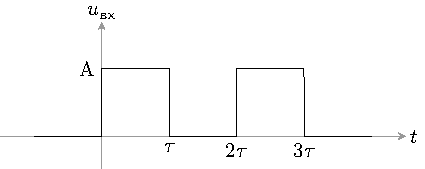
\includegraphics[width=\linewidth]{ris/task12_in}
\caption{Входное напряжение}
\label{fig:4figsB}
\end{minipage}
\qquad
\begin{minipage}{0.35\textwidth}
\centering
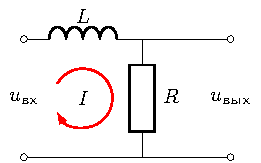
\includegraphics[width=\linewidth]{chem/task2}
\caption{$RL$--контур}
\label{fig:4figsA}
\end{minipage}
\end{figure}

\begin{task}
	Определить отклик $u_\out(t)$ $RL$-цепи, изображенной на рисунке, на воздействие двух прямоугольных импульсов длительностью $\tau$. 
	Нарисуйте график отклика. 
	Какова переходная характеристика цепи? 
	При выполнении какого условия будет осуществляться приближённое интегрирование входной цепи?
	Решить задачу с ненулевыми начальными условиями.
\end{task}
\begin{proof}[\rm{\textbf{Решение}}]
Найдем образ входного импульса преобразованием Лапласа: 
\begin{equation}
	u_\in(t)=A[\H(t)-\H(t- \tau)]+A[\H(t-2 \tau)-\H(t-3 \tau)]
\end{equation}
\begin{equation}
	u_\in(t)\LT \frac{A}{p}\qty(1-e^{-p \tau}+e^{-2p \tau}-e^{-3p \tau})
\end{equation}

Надо учесть, что в контуре могут быть заданы начальные условия - напряжение на индуктивности $u_L(0)=u_0$. Его образ $u_L(0) \LT \frac{u_0}{p} =\frac{i_0\cdot pL}{p}=i_0L$. Это напряжение можно учесть как ещё одну стороннюю ЭДС.

Обозначим суммарный ток в контуре за $I(p)$. Тогда, так как сумма падений напряжения на каждом элементе равна нулю, получим следующее выражение:
\begin{equation}
	u_\in+Li_0=(pL+R)i_0
\end{equation}
Откуда выразим ток $I$:
\begin{equation}
	I(p)=
	\frac{\frac{A}{p}\qty(1-e^{-p \tau}+e^{-2p \tau}-e^{-3p \tau})+Li_0}
	{pL+R}
\end{equation}
После простых алгебраических преобразований получим:
\begin{equation}
	I(p)=
	\frac{\frac AL }{p+\frac{R}{L}}-
	\frac{\frac AL e^{-p\tau}}{p+\frac{R}{L}}+
	\frac{\frac AL e^{-2p\tau}}{p+\frac{R}{L}}-
	\frac{\frac AL e^{-3p\tau}}{p+\frac{R}{L}}+
	\frac{i_0}{p+\frac{R}{L}}
\end{equation}
Отсюда можем получить напряжение на выходе:
\begin{equation}
	u_\out(p)=I(p)\cdot R=
	\frac{A\frac RL }{p+\frac{R}{L}}-
	\frac{A\frac RL e^{-p\tau}}{p+\frac{R}{L}}+
	\frac{A\frac RL e^{-2p\tau}}{p+\frac{R}{L}}-
	\frac{A\frac RL e^{-3p\tau}}{p+\frac{R}{L}}+
	\frac{i_0R}{p+\frac{R}{L}}
\end{equation}
Используем свойства преобразования Лапласа:
\begin{gather}
	\frac{\alpha}{p(p+\alpha)}\LT (1-e^{-\alpha t})\H(t)\\
	\frac{1}{(p+\alpha)}\LT e^{-\alpha t}\H(t)\\
	e^{{-p\tau}}F(p) \LT f(t-\tau)\H(t-\tau), \qq{где} F(p) \LT f(t)
\end{gather}
\begin{figure}[h!]
	\centering
	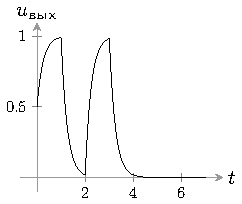
\includegraphics[scale=1.6]{ris/task12_out2}
	\caption{Решение при $A=1, i_0R=0.5, \tau=5, R/L=4, \tau=1$}
	\label{fig:12.2}
\end{figure}
Произведем преобразование:
\begin{gather}
	u_\out (t)=
		A \bigg\{ 
			\qty(1-e^{-\frac{R}{L}t})\H(t)-
			\qty(1-e^{-\frac{R}{L}(t- \tau)})\H(t- \tau)+
			\qty(1-e^{-\frac{R}{L}(t- 2\tau)})\H(t- 2\tau)-\\-
			\qty(1-e^{-\frac{R}{L}(t- 3\tau)})\H(t- 3\tau)
		\bigg\}+
	i_0Re^{-\frac{R}{L}t}\H(t)
\end{gather}



\begin{equation}
	u(t)=(E-u_0)\H(t)\exp{-\frac{t}{CR}}-E \exp{-\frac{t- \tau	}{CR}}\H(t-\tau )
\end{equation} 
График решения при при $A=1, i_0R=0.5, \tau=5, R/L=4, \tau=1$ изображен на рис. \ref{fig:12.2}



\paragraph{Условие интегрирования.} 
Рассмотрим очевидное равенство $u_\in=u_L+u_\out$.
Перепишем это выражение:
\begin{equation}
	u_\in=L\dv{I}{t}+\underbrace{IR}_{u_\out}
\end{equation}
Проинтегрируем его по времени:
\begin{equation}
	\int u_\in \dd{t}=
		\frac{L}{R}\underbrace{IR}_{u_\out}+R\int I \dd{t}
\end{equation}
Если будет выполнено условие
\begin{equation}
	\label{eq:int}
	% \abs{L\dv{u_L}{t}} \ll \abs{\frac{R}{L} u_L} \qquad
	\abs{R\int I \dd{t}} \ll \abs{LI} \quad \Rightarrow \quad
	\abs{\int I \dd{t}} \ll \abs{\frac{L}{R}I}
\end{equation}
То выходное напряжение с точностью до множителя интегрирует входное:
\begin{equation}
	u_\out=\frac{1}{\tau_\text{цепи}}\int u_\in \dd{t}
\end{equation}
где $\tau_\text{цепи}=\frac{L}{R}$.

Выясним смысл неравенства модулей на примере гармонических сигналов. Пусть входное напряжение гармоническое $u_\in=u_0e^{j\omega t}$. Тогда ток в контуре: $I=I_0e^{j\omega t}$, где $I_0=\frac{u_0}{j\omega L+R}$, и неравенство (\ref{eq:int}) можно переписать:
\begin{equation}
	\abs{I_0\frac{1}{j\omega}e^{j\omega t}}\ll
		\abs{{\tau_\text{цепи}}I_0e^{j\omega t}}
	\quad \Rightarrow \quad
	\frac{1}{\omega} \ll {\tau_\text{цепи}}
	\quad \Rightarrow \quad
	T \ll \tau_\text{цепи}
\end{equation}
Таким образом, интегрирование сигнала <<чистое>> для таких частот, период которых много меньше постоянной цепи. Отсюда следует <<вилка выбора>> интегрирующей цепочки: если мы будем расширять частотный диапазон <<чистого>> интегрирования, то амплитуда на выходе цепочки будет падать, и наоборот.

\end{proof}
\end{document}
